\documentclass{article}
\usepackage{FinalYearProjectReport}

% uncomment this line to double line spacing for proof reading
% \linespread{2}

% packages and settings for graphics
\usepackage[pdftex]{graphicx}
\graphicspath{{./}}
\DeclareGraphicsExtensions{.png}
\usepackage[final]{pdfpages}

\setlength\paperheight{297mm}
\setlength\paperwidth{210mm}

\usepackage{avant}
\renewcommand{\familydefault}{\sfdefault}
\frenchspacing

\title{Mini Project Final Report}
\name{Adil \textsc{Bhayani} \& Sakayan \textsc{Sitsabesan}}
\address{Department of Electrical and Computer Engineering\\
University of Auckland, Auckland, New Zealand}

\begin{document}

\begin{titlepage}

\newcommand{\HRule}{\rule{\linewidth}{0.5mm}} % Defines a new command for the horizontal lines, change thickness here

\center % Center everything on the page
 
%----------------------------------------------------------------------------------------
%	HEADING SECTIONS
%----------------------------------------------------------------------------------------

\textsc{\LARGE University of Auckland}\\[1.5cm] % Name of your university/college
\textsc{\Large COMPSYS 305: Digital Systems Design 1}\\[0.5cm] % Major heading such as course name
\textsc{\large Mini Project }\\[0.5cm] % Minor heading such as course title

%----------------------------------------------------------------------------------------
%	TITLE SECTION
%----------------------------------------------------------------------------------------

\HRule \\[0.4cm]
{ \huge \bfseries Final Report}\\[0.4cm] % Title of your document
\HRule \\[1.5cm]
 
%----------------------------------------------------------------------------------------
%	AUTHOR SECTION
%----------------------------------------------------------------------------------------

\begin{minipage}{0.4\textwidth}
\begin{flushleft} \large
\emph{Author:}\\
Adil \textsc{Bhayani} \newline
Sakayan \textsc{Sitsabesan}
\end{flushleft}
\end{minipage}
~
\begin{minipage}{0.4\textwidth}
\begin{flushright} \large
\emph{Supervisor:} \\
Dr. Muhammad \textsc{Nadeem} % Supervisor's Name
\end{flushright}
\end{minipage}\\[1cm]


%----------------------------------------------------------------------------------------
%	DATE SECTION
%----------------------------------------------------------------------------------------

{\large \today}\\[2cm] % Date, change the \today to a set date if you want to be precise

%----------------------------------------------------------------------------------------
%	LOGO SECTION
%----------------------------------------------------------------------------------------

\includegraphics{uoa.jpg}\\[1cm] % Include a department/university logo - this will require the graphicx package
 
%----------------------------------------------------------------------------------------

\vfill % Fill the rest of the page with whitespace

\vspace*{25em}

{\Large Declaration of Originality}

\hspace{5em}

This report is our own unaided work and was not copied from 
nor written in collaboration with any other person.

Name: Adil \textsc{Bhayani} \& Sakayan \textsc{Sitsabesan}


\end{titlepage}




\maketitle

\begin{abstract}

The Mini Project consists of designing a game on a FPGA device which incorporates one simple tank defence game called Tank Hunting. The overall objective is to learn the process of digital design and logic by practically applying the skills learnt prior to the project.

\end{abstract}

\section{Introduction}

Tank hunting is a game that revolves around the player defending their own tank while shooting as many enemy tanks as possible within the time frame. The game consists of 3 levels of increasing difficulty. The player must manoeuvre their tank at the bottom of the screen to effectively shoot the enemy tanks at the top of the screen and increase their score. The player is required to dodge enemy bullets and stop tanks from reaching their base at the bottom of the screen.

Many components were provided to us as the mouse, char ROM and a partial implementation of tank. As part of our contribution to the game we have added code for the various components such as game, counter and SSD alongside significant code additions to the tank file. In terms of features we have added elements such as menu screens after each level to display the score to the user. As well as the ability for the enemy tanks to shoot back at the player and slowly make their way down to the bottom of the screen which the player must defend. In the last level, we have also added the feature of limiting the players bullets to fifteen but allowing the user to gain back bullets by successfully hitting enemy tanks.

\section{Design Specification}

\subsection{Available Equipment}

The following set of equipment has been provided for this project:

\begin{itemize}
\item DE0-Board
\item PS/2 Mouse
\item VGA Cable
\end{itemize}

\subsection{Design Definition and Requirements}

Tank Hunting is a simple 2D shooter game that revolves around controlling one tank to effectively destroy as many AI controlled tanks within a set time frame per level (game mode). The DE0 board which is acting as the console must interface with a monitor through a VGA cable to display a screen with a resolution of 640 x 480 pixels. The player will interface with the system through the DIP switches and buttons available on the board and through inputs from the PS/2 mouse.

The AI is to be designed so that the tank is bouncing on the edges of the screen in a horizontal line. The movement of the bottom tank is player controlled through the mouse and bullets can be shot by pressing the left mouse button. Both tanks must have two distinct colours. A bullet can only be shot when the other bullet has left the screen or when an AI tank has been hit. When a tank is hit, it must disappear and then reappear in a seemingly random x position while the player’s score should increase. Once all three levels have been cleared the game can be reset using the earlier mentioned buttons.

The levels should be designed in a manner which demonstrates increasing difficulty. This is achieved by increasing the speed of the AI controlled tanks and changing bullet speeds, alongside the implementation of additional features. 

\subsection{Optional Tasks and Additional Feature Design}

The first AI tank has be given the ability to shoot back at the player’s tank in the third level. If the playe'rs tank is hit then the game will end. Additionally, a secondary tank has been added which will begin to move down towards the player. The game will also end if this tank goes off the screen or collides with the player’s tank. 

The set of requirements listed above are essential minimums and form a general guideline for the design of the system. To improve gameplay and to make the game more challenging additional features are to be implemented and incorporated in a manner which allows the game to flow and become increasingly difficult as levels are cleared. These will be discussed in greater detail in game strategy.

\section{Block Diagram}

\begin{figure}[!h]
\centerline{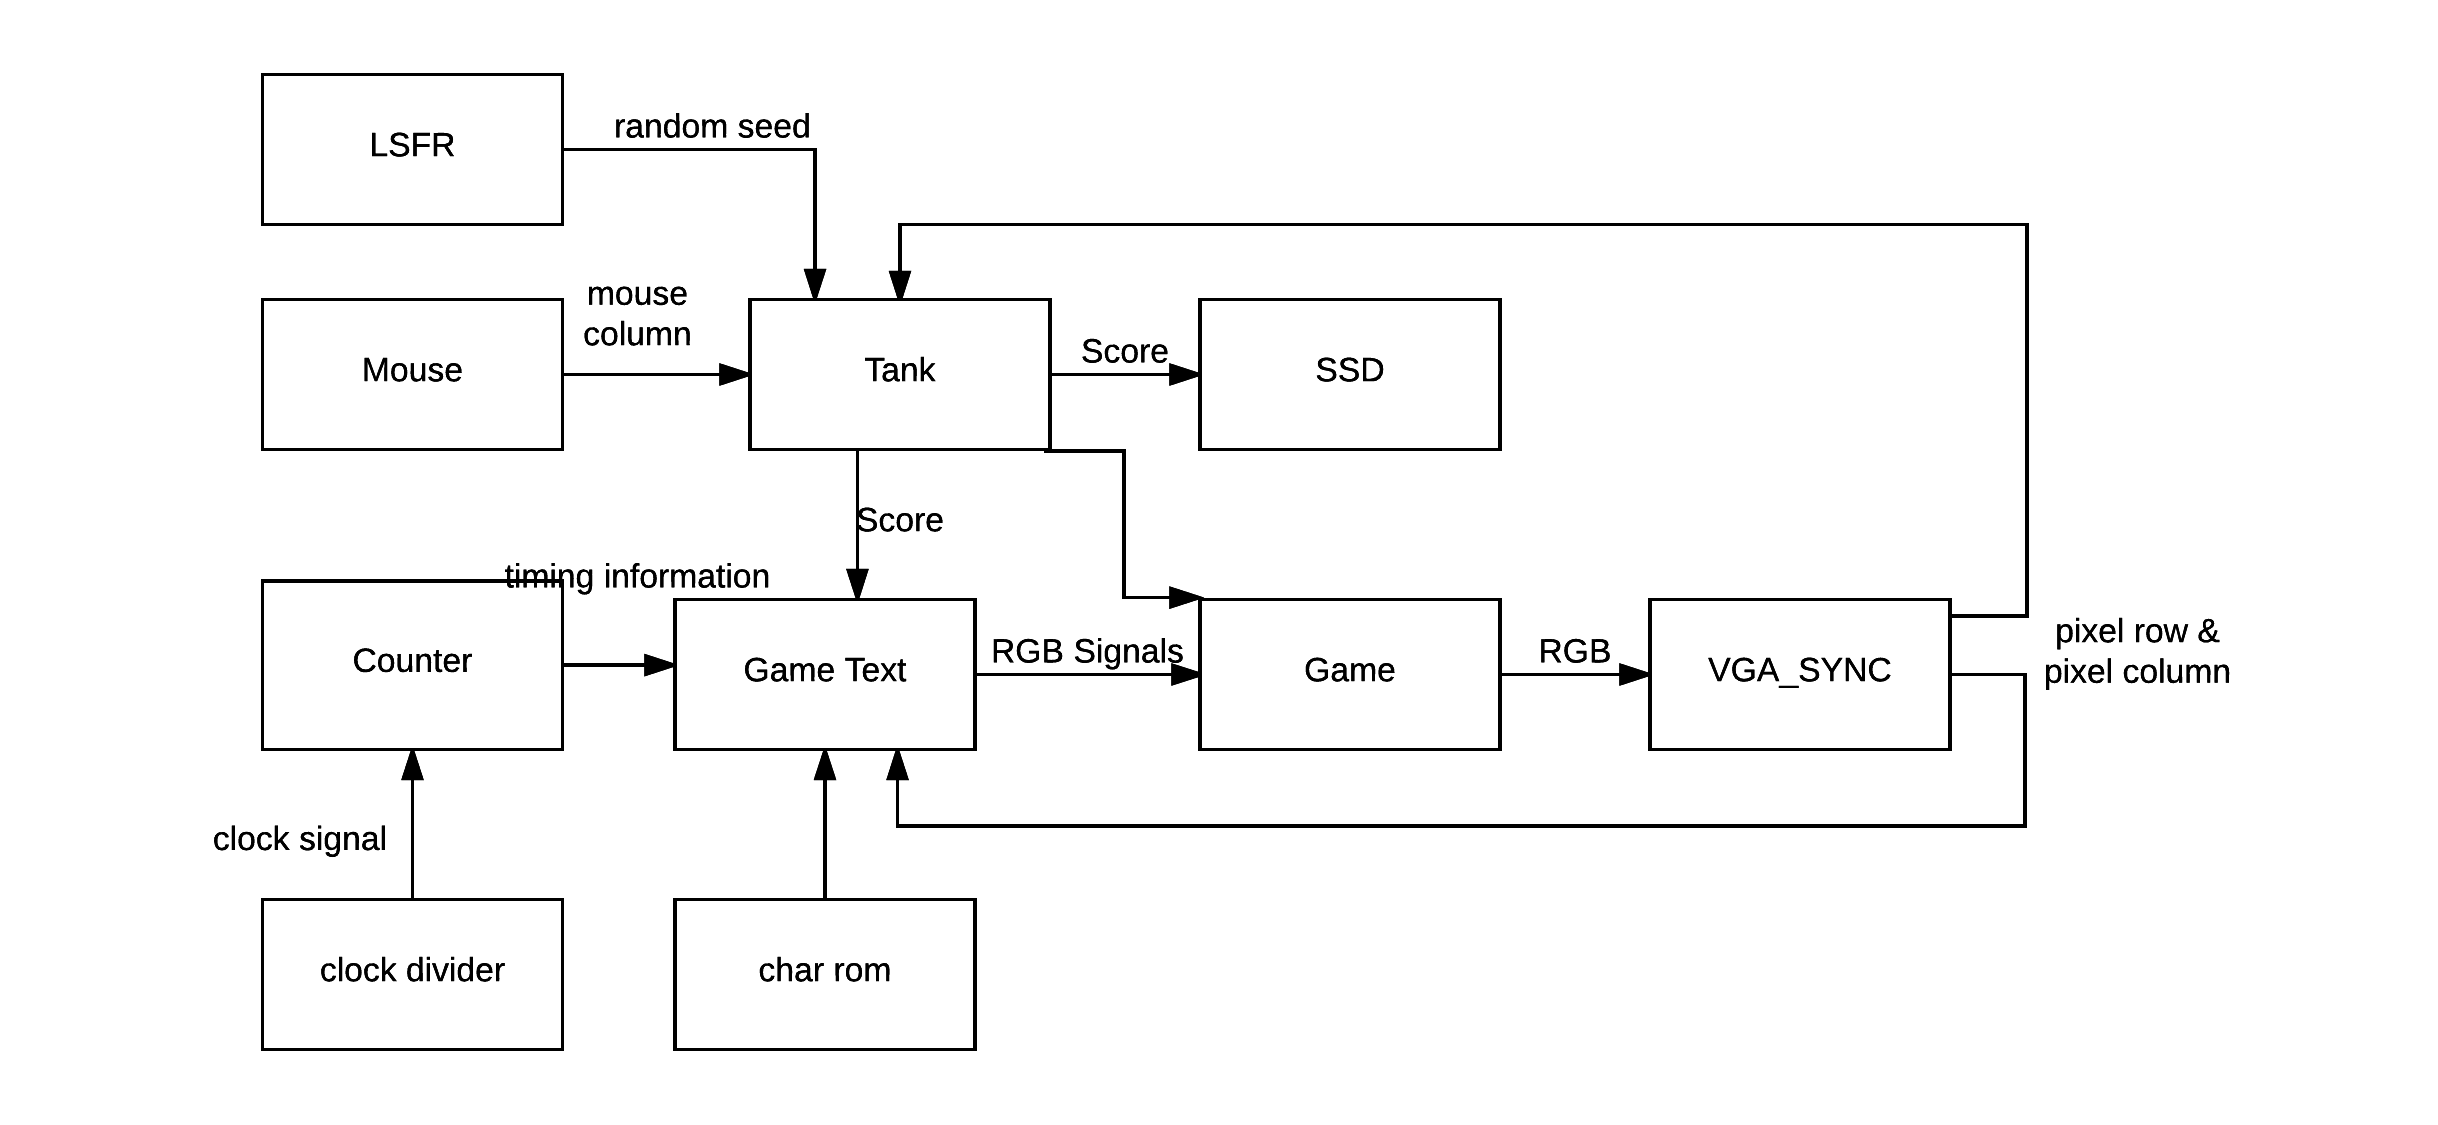
\includegraphics[width=0.5\textwidth]{block_diagram}}
\caption{Block Diagram}
\label{fig:rawFrame}
\end{figure}

\quad\textbf{LSFR:} The LSFR generates a random seed for the starting location of AI tanks. The output is a eleven bit number.

\textbf{Mouse:} Manages all signals sent to and from the mouse. The mouse column data and the button click data is passed on to the Tank entity which process the data.

\textbf{Clock Divider:} Divides the 50Mhz clock signal down to 1Hz for the counter to count in seconds.

\textbf{Counter:} Countdown timer for the game levels to time the lenght of the levels. Output is passed for rendering by Game Text entity.

\textbf{Char ROM:} Stores the pixel information for rendering text in the game. Accessed by the Game Text entity.

\textbf{Game Text:} Generates the appropriate text for the current screen and passes the output to the game entity for it to be muxed into the VGA signal.

\textbf{Tank:} The Tank entity to control movement, shooting and score of tanks. Inputs from mouse, LSFR \& game. Outputs the score to the Seven segment decoder and game text aas well as outputing the RGB signals to the game entity.

\textbf{Seven Segment Decoder:} Decodes the scores and mouse column packet data and outputs it to the seven segment decoder.

\textbf{Game:} Manages the game scene to render and muxes in the appropriate signals from the game text and tank entities. Uses an FSM to manage game state.

\textbf{VGA\_Sync:} Syncs the VGA signal to be sent out of the VGA port to the monitor. VGA sync signals are looped back to the Game Text and Tank entity for alligning the pixels on the screen.

\section{Game Strategy}

The main objective of the game is to complete all three levels without losing as well as to get the highest score possible. Since the game will consist of three levels that will be of increasing difficulty, transitions will happen after the specified time has been reached. This allows the player to maximise their score by playing until the time limit has been reached. Once a level has been cleared the player's score will be shown on the screen as an intermediate progress screen, which can also be customised to incorporate a story. By interacting with the push buttons the player can continue to the next level. The score will be retained across all levels allowing the player to accumulate their score and aim for a new high score.

\subsection{Level 1}

The first level only has one AI controlled tank that moves slowly across the top of the screen. The player is be able to move across the screen faster than the AI and can easily score many points considering the bullet speed is also very high.

\subsection{Level 2}

This level brings in the addition of the second tank and increases the speed of both AI tanks. The player's tank speed remains unchanged to increase the difficulty. A restriction has be placed on the number of bullets that the player can shoot, with the ability to get back bullets by successfully hitting an AI tank.

\subsection{Level 3}

The final level of the game has been designed to be truly challenging. Alongside the increased AI tank speed, one tank will now move downwards towards the player’s tank while the other will shoot back at the player. If a bullet hits the player the game will immediately end. Similarly, collisions between the downward moving AI tank and the player’s tank or the AI tank moving off the screen downwards will also cause the game to end. This means that the player will now have to actively defend themselves while attempting to increase their score. Bullet restrictions will remain, similar to level two. 

\section{Final System Design \& Implementation}

The Finite State Machine is composed of eight states; 000, 001, 010, 011, 100, 101, 110, 111. These represent the Main Menu, Practice Mode, Level 1 Game, Level 1 End Screen, Level 2 Game, Level 2 End Screen, Level 3, Level 3 End Screen respectively. 

The finite state machine is used in this implementation to track which level of the game the user currently is in and output the appropriate game graphics and text to the screen as well as set the bullet counters and timers to the appropriate values. The FSM controls the final mux of the video signals before they are output to the display through the VGA\_Sync component. 

This FSM and mux are all part of the `game' component of this implementation. No game logic/collisions/etc. has been implemented in this component. That is all handled by the `tank' component.

\begin{figure}[!h]
\centerline{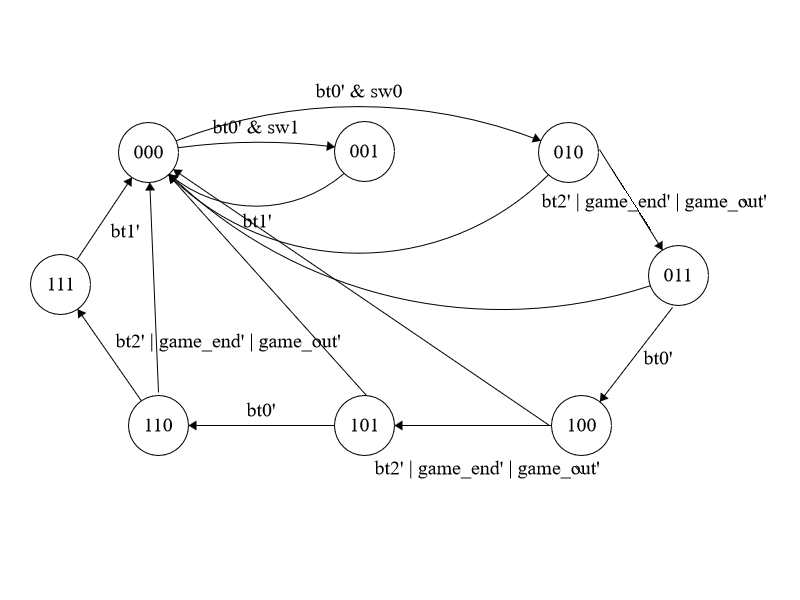
\includegraphics[width=0.5\textwidth]{fsm}}
\caption{Finite State Machine}
\label{fig:rawFrame}
\end{figure}

The `tank' component is the main component in this implementation and handles most of the game related logic in this project. The `tank' component consists of two processes; a RGB\_Display Process \& a Move\_Tank Process. The RGB display process operates on input signals Tank\_on, Bonus\_on, Player\_on, Bullet\_on \& Special\_on. These signals are produced by the Move Tank process and are set to `1' when they are located on the current pixel. The RGB Display process converts these signals with the pre-set size variables to 4-bit RGB colours for displaying on the screen.

The Move\_Tank process is responsible for converting the mouse inputs into tank movements and controls the appearence and movements of the bullets. When the FSM changes into any of the game level states, the Move Tank process resets itself, and the player tank starts at the centre bottom, AI Tank starts are random location and moves in random direction based on the inputs from the LSFR, which generates a psuedorandom number. 

The bullets are initally invisble and located at the centre of the screen when the game begins. When the player fires a bullet, it is moved to the current location of the tank, made visible and set to move at a constant rate upwards. This constant rate is determined by the game level, so as to increase in game difficulty with the game levels.

In the second game level, a second AI tank also appears along the top of the screen. This second tank mirrors the position of the first tank. In the third game level, the second tank also starts moving downwards slowly at a constant rate. In addition, the first tank starts shooting bullets whenever the 5th bit of the LSFR is `1' and there is currently no AI bullet in play. Similar to the player bullet, this bullet is initally inivisible and becomes visible and moves to the tank's location when a bullet is shot.

When a bullet passes through the pixels of an enemy tank, the bullet is moved to the centre of their side of the screen and made invisible. Collision detection of that bullet is also disabled when the bullet is invisible. This approach is necessary as the resources on the FPGA can not be allocated dynamically at run-time and must instead be statically allocated when the FPGA is programmed.

Whenever the pause switch is switched on, everything in the Move\_Tank process \& counter are stopped. The main FSM continues to run so that the user may exit from the game while it is paused.

The counter is a basic down counter that counts down from 99 to 0. The remaining components are generic components which are not particular to this project, some of which were supplied for use in this project.

\section{Design Decisions}

In our design, the functionality of the design and their attributes are managed by only the Tank component as opposed to having multiple components for different tanks and their features. This allowed us to maximise code re-use while minimising the amount of wiring required between the additional components. The trade off to this was that our Tank component is slightly more complicated than the components which would have been present if the Tank component was broken up into smaller parts. However, the Tank component is still sufficiently simple to understand and work with, justifying the design decision.

\section{Performance}

\begin{figure}[!h]
\centerline{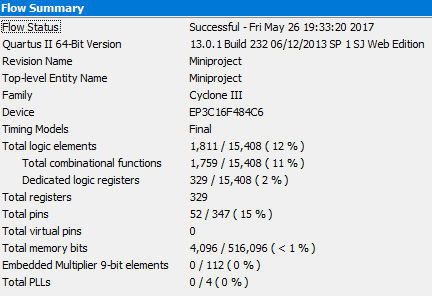
\includegraphics[width=0.5\textwidth]{flow_summary}}
\caption{Flow Summary}
\label{fig:rawFrame}
\end{figure}

A total of 4096 of the 516,096 memory bits available on the on chip memory has been used in this project. This is used to store the character ROM for rendering the ASCII characters on the screen. This was the only data that was stored in the dedicate memory part of the FPGA. This memory was loaded as read only at initialization from a MIF file that was supplied. A total of 52 pins are used to connect to the various I/O sources used in the project, the majority of these are for the seven segment display (7 x 4) and the VGA output (3 x 4). 

The project implementation occupies a total of 1811 Logic elements in the Cyclone III FPGA, of these 1759 are combinational functions and the remaining 329 are dedicated logic registers. Switching from 1-bit to 4-bit graphics significantly (40\%) increased the number of logic elements used in the design. This increase was seen as worthy of the graphics improvement it provided and as a result the final design used 4-bit graphics.

The maximum opertating frequency of the implementation is 130.46MHz, this a restriction caused by the vert\_sync\_out signal from the VGA SYNC component to the tank entity. This restriction can be alieviated by the putting registers between on this signal line and making the critical path shorter. The maximum operating frequency of this design is much greater than the clock frequncy of the FPGA we are using the DE0 and is therefore ideal.

\section{Discussion \& Future Works}

Our mini project was to create a Tank Hunting game implemented with a FPGA device as a console. The game was displayed on a screen through a VGA cable at a resolution of 480 x 640. Our final game consisted of three levels of increasing difficulty. The screen shows the user information such as the game level, their score and the time remaining for the level. The game was designed to be challenging yet playable to allow the player to consistently strive for a new high score in each play through.

If given more time for the project, in future iterations we would implement additional features alongside improved graphics and sound effects. Additional features would include multiplayer abilities by integrating inputs from the keyboard to control a secondary tank which would replace the AI tanks in a third multiplayer game mode. We would also add the ability to have powerups like sped up bullets or allowing a tank to become invincible for a certain amount of time. The aim of adding these additional features would be to increase the playability of the game and to ultimately make the game more fun.

\clearpage

\section{Appendices}

\subsection{Extended Block Diagrams}

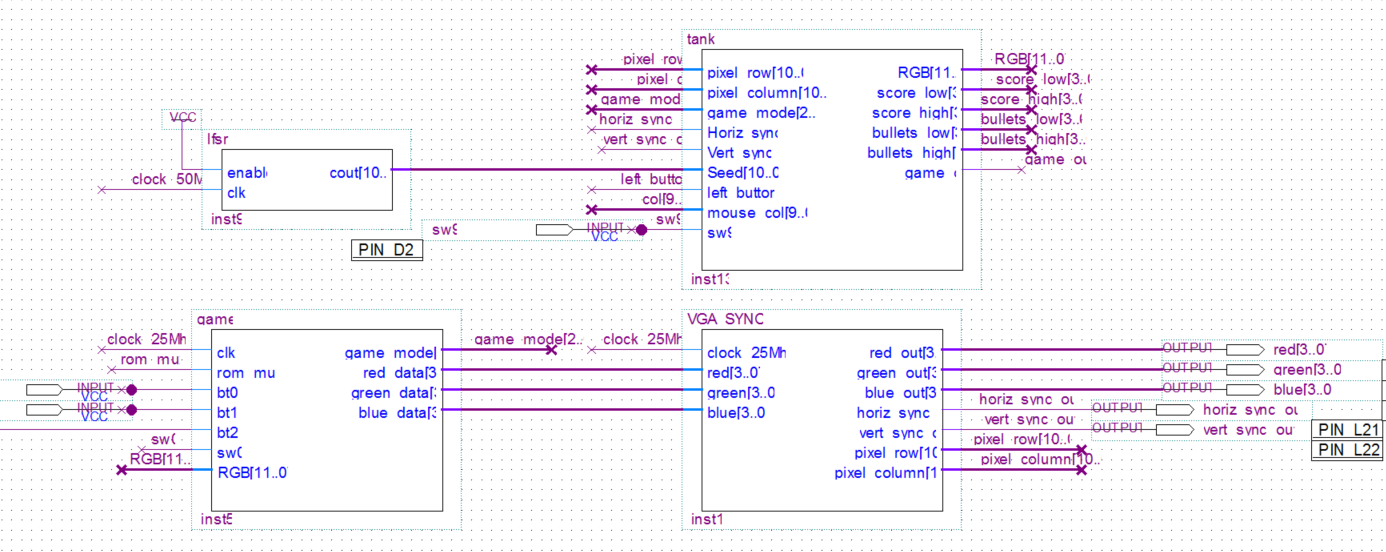
\includegraphics[width=1\textwidth]{appendix1.png}

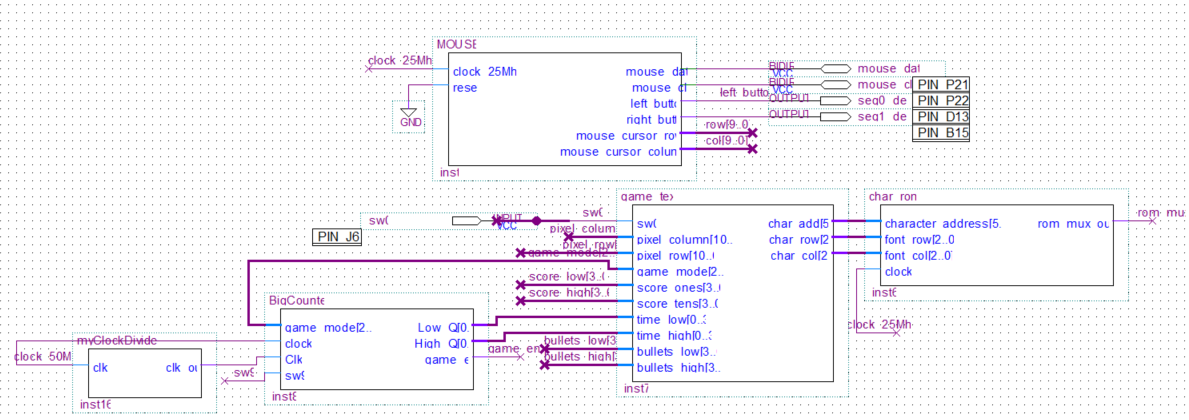
\includegraphics[width=1\textwidth]{appendix2.png}

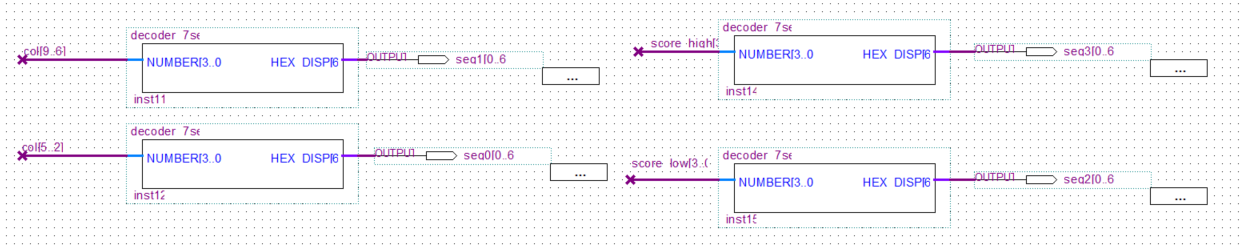
\includegraphics[width=1\textwidth]{appendix3.png}

\end{document}